\documentclass{sig-alt-full}
%\documentclass[10pt]{article}
%\usepackage{times}
%\usepackage{fullpage}
\usepackage[noend]{algpseudocode}
\usepackage{amsmath}
%\usepackage{amsthm}
\usepackage{seanmacros}
\usepackage{multicol}
\usepackage{bm}

%\pdfpagewidth=8.5in
%\pdfpageheight=11in

%%%%% Force single space for now

%\makeatletter
%Remove ACM copyright notice at the lower left corner
%\renewcommand{\@copyrightspace}{}
%Make the ACM template into single column
%\renewcommand{\twocolumn}[1][1]{\onecolumn #1}
%\makeatother

%%%%% End Force single space

\newtheorem{theorem}{Theorem}
\newtheorem{lemma}{Lemma}
\newtheorem{algorithm}{Algorithm}
\newtheorem{defn}{Definition}

%%%%%% Make a strut
\newcommand\strt{\rule{0pt}{1.8em}}


% macro to overlap math
\def\clap#1{\hbox to 0pt{\hss#1\hss}}
\def\mathllap{\mathpalette\mathllapinternal}
\def\mathrlap{\mathpalette\mathrlapinternal}
\def\mathclap{\mathpalette\mathclapinternal}
\def\mathllapinternal#1#2{%
	\llap{$\mathsurround=0pt#1{#2}$}}
\def\mathrlapinternal#1#2{%
	\rlap{$\mathsurround=0pt#1{#2}$}}
\def\mathclapinternal#1#2{%
	\clap{$\mathsurround=0pt#1{#2}$}}

\newcommand\proda[1]{\displaystyle\prod_{#1}}
\newcommand\prodb[2]{\displaystyle\prod_{\stackrel{{#1} :}{#2}}}
\newcommand\prodc[1]{\prod_{#1}}
\newcommand\prodd[2]{\prod_{#1}^{#2}}
\newcommand\suma[1]{\displaystyle\sum_{#1}}
\newcommand\sumb[2]{\displaystyle\sum_{\stackrel{{#1} :}{#2}}}
\newcommand\sumc[1]{\sum_{#1}}
\newcommand\sumd[2]{\sum_{#1}^{#2}}
\newcommand\laxsumb[2]{\displaystyle\sum_{\mathclap{\stackrel{{#1} :}{#2}}}}
\newcommand\smashedsumb[2]{\smash{\displaystyle\sum_{\mathclap{\stackrel{{#1} :}{#2}}}}}

\begin{document}

\conferenceinfo{FOGA'09,} {January 9--11, 2009, Orlando, Florida, USA.} 
\CopyrightYear{2009}
\crdata{978-1-60558-414-0/09/01} 

%\pagestyle{plain}
%\pagenumbering{arabic}   %%% force page numbering
%\normalsize

\title{Cooperative Coevolution and Univariate \\Estimation of Distribution Algorithms}

\numberofauthors{3}
\author{
Christopher Vo\\
       \affaddr{Dept. Computer Science}\\
       \affaddr{George Mason University}\\
       \affaddr{4400 University Dr., MSN 4A5}\\
       \affaddr{Fairfax, VA 22030}\\
       \email{cvo1@gmu.edu}
\alignauthor
Liviu Panait\\
       \affaddr{Google, Inc.}\\
       \affaddr{604 Arizona Avenue}\\
       \affaddr{Santa Monica, CA 90401}\\
       \email{liviu@google.com}
\alignauthor
Sean Luke\\
       \affaddr{Dept. Computer Science}\\
       \affaddr{George Mason University}\\
       \affaddr{4400 University Dr., MSN 4A5}\\
       \affaddr{Fairfax, VA 22030}\\
       \email{sean@cs.gmu.edu}
}
%\date{}
\maketitle

\begin{abstract}
In this paper, we discuss a curious relationship between Cooperative Coevolutionary Algorithms (CCEAs) and univariate Estimation of Distribution Algorithms (EDAs).  Specifically, the distribution model for univariate EDAs is equivalent to the infinite population EGT model common in the analysis of CCEAs. This relationship may permit cross-pollination between these two disparate fields. As an example, we derive a new EDA based on a known CCEA from the literature, and provide some preliminary experimental analysis of the algorithm.
\end{abstract}

% A category with the (minimum) three required fields
\category{F.2}{Theory of Computation}{Analysis of Algorithms and Problem Complexity}
\category{G.1.6}{Optimization}{Global Optimization}

\terms{Theory, Algorithms}

\keywords{Cooperative Coevolution, Estimation of Distribution Algorithms, Evolutionary Game Theory}

%\normalsize

\section{Introduction}

We describe a relationship between two seemingly unrelated corners of the evolutionary computation community: Cooperative Coevolutionary Algorithms (CCEAs) and univariate Estimation of Distribution Algorithms (EDAs).  These two families of algorithms were independently proposed and developed.  Cooperative coevolution has emerged as a mechanism to simplify the search space by projecting it into multiple smaller subspaces, each searched by a separate population; whereas EDAs have often been proposed as competitors with ``traditional'' sample-based EAs, by replacing the sample population with a distribution estimate.  In particular, univariate Estimation of Distribution Algorithms represent the population distribution as a collection of separate per-gene distributions.

As it turns out, these algorithms have a strong but non-intuitive relationship. The per-gene distributions of univariate EDAs are not only closely related to the multiple populations of CCEAs, but such distributions are in fact {\it equivalent to} the infinite-sized ``populations'' used in a very common theoretical model for CCEAs, one based on Evolutionary Game Theory (EGT).  This relationship promises to yield cross-pollination between the two fields: CCEAs have lately built a strong theoretical formulation; and EDAs have both good theory and efficient algorithms.  We hope that this paper kindles discussion between the two fields. 

We begin the paper by first discussing CCEAs and relevant theory.  We then discuss univariate EDAs and outline one well-known univariate EDA algorithm as an example. We then formally show the relationship between the two.  Based on this relationship, we offer an example of direct transfer from one area to the other: namely, we introduce a new theoretical univariate EDA formulation derived from a CCEA EGT model.  We prove that the algorithm can converge to the optimum with any desired probability, though it is not efficient compared to existing EDA algorithms.  We also provide an actual EDA algorithm which is an approximation of the theoretical version.


\section{Cooperative Coevolution}

Coevolutionary algorithms generally assign fitness to an individual not based on an absolute measure but rather on the interaction of that individual with other individuals in the evolutionary system.  The hallmark of a coevolutionary algorithm is that the relative order of any two individuals may change depending on the presence of those other individuals in the system.

\ignore{The most common coevolutionary frameworks are {\it one-population competitive}, {\it two-population competitive}, and {\it n-population cooperative} arrangements.  In the one-population competitive coevolutionary algorithm, individuals in a single population are assessed by pitting them against other individuals in the same population, often in a game (for example, evolving checker players \cite{chellapilla99evolving}).  In the two-population competitive arrangement, individuals from one population are pitted against individuals against an opposing population. Here, typically only one population contains solutions of interest to the experimenter; the second population serves as a foil to push the first population towards robust solutions (for example, a sorting networks versus sorting problems \cite{Hillis91}).}

In this paper, we focus on {\it n-population cooperative} arrangements, popularly known as Cooperative Coevolutionary Algorithms (CCEAs) \cite{Potter94,Potter00}.  In CCEAs, the solution space is broken into some {\it n} sub-solution spaces, and each sub-solution space is assigned a population.  An individual is assessed by grouping it with individuals from the other populations to form a complete solution; the quality of this solution is then incorporated into the individual's fitness.  Cooperative coevolutionary algorithms can be generational or steady-state, and often take one of two forms: {\it serial} versus {\it parallel} algorithms.\ignore{In a serial algorithm, each population is evaluated and updated in turn, round-robin.  In the parallel algorithm, all of the populations are evaluated before any of them is bred.} One common parallel generational CCEA may be described as:

\vspace{1in}

{\it{\sc Algorithm 1:} Parallel Generational CCEA}
\begin{algorithmic}[0]
\Loop\hspace{\fill}
	\For{each population \(p \in P\)}
		\For{each individual \(i \in p\)}
			\State Evaluate(\(i, p, P\))
		\EndFor
	\EndFor
		\vspace{-0.25em}
	\For{each population \(p \in P\)}
		\State Breed whole population \(p\)
	\EndFor
\EndLoop
\end{algorithmic}


\ignore{
\vbox{
\label{serialgenerational}
\vspace{1em}
\begin{algorithmic}[0]
\Loop \hspace{\fill} {\it ({\sc Algorithm 0.} Serial Generational CCEA)}
	\For{each population \(p \in P\)}
		\For{each individual \(i \in p\)}
			\State Evaluate(\(i, p, P\))
		\EndFor
		\vspace{-0.25em}
	\State Breed whole population \(p\)
	\EndFor
\EndLoop
\end{algorithmic}
}
}

\ignore
{
The algorithms may also be steady state, again either serial or parallel.  Here, only one (or a few) individuals from each population are updated at a time, rather than all the individuals.  Ignoring the initialization procedures, the steady-state loops are roughly:

\vbox{
\vspace{1em}
\begin{algorithmic}[0]
\Loop \hspace{\fill} {\it ({\sc Algorithm 2.} Serial Steady-State CCEA)}
	\For{each population \(p \in P\)}
		\State Breed an individual \(i\)
		\State Evaluate(\(i, p, P\))
		\State Introduce \(i\) into \(p\), discarding another
	\EndFor
\EndLoop
\end{algorithmic}
}

{
\vspace{1em}
\begin{algorithmic}[0]
\Loop \hspace{\fill} {\it ({\sc Algorithm 3.} Parallel Steady-State CCEA)}
	\For{each population \(p \in P\)}
		\State Breed an individual \(i_p\)
		\State Evaluate(\(i_p, p, P\))
	\EndFor
		\vspace{-0.25em}
	\For{each population \(p \in P\)}
		\State Introduce \(i_p\) into \(p\), discarding another
	\EndFor
\EndLoop
\end{algorithmic}
}
}

Much of cooperative coevolution research has focused on the specifics of the Evaluate(\(i,p,P\)) function.  Choice of evaluation procedure in CCEAs is known to lead to pathologies.  Certain of these have been studied at length using a theoretical model for CCEAs which, while somewhat different from actual CCEAs, provides insight into their dynamics.  We discuss this model next.

\subsection{The Evolutionary Game Theory Infinite Population Model}
\label{egt}

Analyses of cooperative (and other) coevolution will often make use of an infinite population formulation derived from evolutionary game theory (EGT).  This formulation usually assumes that each population is infinite in size, but is drawn from a finite set of genotypes. Much EGT work in cooperative coevolution has focused on two populations.  The first population is represented by a vector \(x\) where \(x_i\) indicates the proportion of genotype \(i\) in the population.  The second population is represented by the vector \(y\).  There also exists a matrix \(A\) whose elements \(a_{ij}\) represent the reward when genotypes \(i\) (from the first population) and \(j\) (from the second population) are combined to form a joint solution.

One common EGT model breaks the evolutionary process into two parts.  First, the fitness of each individual is assessed. We will use the vector \(u\) to represent the fitness of the genotypes in the first population such that each genotype \(i\) has fitness \(u_i\).  Likewise, we will use \(w\) for the second population.  Wiegand \cite{Wiegand2003phd} defined the fitness of a genotype as the average reward received when pairing it with {\it every} member of the other population.  That is, at time \(t\):
%
\begin{align}
\label{egtfitness}
u_i^{(t)} &= \sum_j a_{ij} y_j^{(t)} &
w_j^{(t)} &= \sum_i a_{ij} x_i^{(t)}
\end{align}

Second, we then update the genotype proportions for the next generation (time \(t+1\)) using a formulation that simulates fitness-proportional selection:

\begin{align}
\label{eqtupdate}
x_i^{(t+1)} &= x_i^{(t)} \left( \frac{u_i^{(t)}}{\sum_k x_k u_k^{(t)}} \right) &
y_j^{(t+1)} &= y_j^{(t)} \left( \frac{w_j^{(t)}}{\sum_k y_k w_k^{(t)}} \right)
\end{align}

Wiegand found that this ``complete mixing'' model could converge towards local suboptima surrounding Nash Equilibria in the joint space: if a suboptimum basin were large and broad, the system would collect at its peak rather than at another taller but narrower peak centered at a global optimum.  This was largely because the fitness procedure {\it averaged} the performance of an individual over {\it all} individuals in the corresponding population, without regard to how good collaborators those corresponding individuals were.\ignore{That is, the fittest individuals tended to be jacks-of-all-trades, doing reasonably well with the average collaborator, rather those which performed optimally when paired with the optimal collaborator (but perhaps poorly on average).} Wiegand termed this pathology {\it relative overgeneralization}.

Later research has shown that the system {\it will} converge if we change the fitness assessment procedure.  One solution is to base the fitness of individuals in a population not on average collaboration but rather on the maximum performance over all collaborations.  Following Panait \cite{panait06analysis} we might change Equation \ref{egtfitness} to:
%
\begin{align}
\label{panaitfitness}
u_i^{(t)} & = \max_j a_{ij} &
w_j^{(t)} &= \max_i a_{ij}
\end{align}

Panait provided a proof of convergence to the optimum \cite{panait06analysis} using this in combination with tournament selection rather than fitness-proportional selection, assuming that the optimum is unique.
%\footnote{Though it is of less relevance to the thrust of this paper, we also have an unpublished proof of convergence using the fitness-proportional selection Equation \ref{eqtupdate}.}  
Panait's derivation of tournament selection (of tournament size \(H\)) transformed Equation \ref{eqtupdate} to:
%
\begin{equation}
\label{tournamentselection}
\begin{split}
x_i^{(t+1)} &= x_i^{(t)} \frac{\left(\sum_{\forall k : u_k^{(t)} \leq u_i^{(t)}} x_k^{(t)} \right)^H \!\!\! - \left( \sum_{\forall k : u_k^{(t)} < u_i^{(t)}} x_k^{(t)} \right)^H} {\sum_{\forall k : u_k^{(t)} = u_i^{(t)}} x_k^{(t)}} \\
y_i^{(t+1)} &= y_j^{(t)} \frac{\left( \sum_{\forall k : w_k^{(t)} \leq w_j^{(t)}} y_k^{(t)} \right)^H \!\!\!\! -\left( \sum_{\forall k : w_k^{(t)} < w_j^{(t)}} y_k^{(t)} \right)^H}{\sum_{\forall k : w_k^{(t)} = w_j^{(t)}} y_k^{(t)}} \\
\end{split}
\end{equation}

This curious equation is a result of the order statistics to compute the expected maximum over a set of size \(H\).  In each subequation there are two terms raised to \(H\) each.  These compute the probability that, of a tournament of size \(H\), the winners (there may be ties) will include a genotype whose fitness is the same as genotype \(i\).   The first term gives the probability that all \(H\) tournament entrants will have a fitness less than or equal to \(i\)'s fitness, and the second term gives the probability that all will have a fitness less than that of \(i\).  The denominators in each subequation compute the probability that the first such winner is in fact \(i\), as opposed to other fitness-equivalent genotypes.

So far, these theoretical models are fairly divorced from real-world CCEAs: the population is infinite; there is no breeding, only selection; and the evaluation procedure involves scanning across all possible collaborators.   But this situation may be improved somewhat.  Panait et al. \cite{panait08theoretical} provided a weakened convergence proof for a more realistic evaluation procedure: take the maximum performance when paired \(N\) times with randomly chosen collaborators.  The proof shows that for any probability \(\epsilon\), there exists an \(N_\epsilon\) such that given \(N_\epsilon\) evaluations, the algorithm is guaranteed to achieve convergence to the global optimum with probability \(1-\epsilon\), when coupled with tournament selection.

The maximum-of-\(N\) evaluation procedure, which replaces Equations \ref{egtfitness} or \ref{panaitfitness}, is:
%
\begin{equation}
\label{maxofn}
\begin{split}
u_i^{(t)} &= \sum_j a_{ij} y_j^{(t)} \frac{\left( \sum_{\forall k : a_{ik} \leq a_{ij}} y_k^{(t)} \right)^N \!\!\! -\left( \sum_{\forall k : a_{ik} < a_{ij}} y_k^{(t)} \right)^N} {\sum_{\forall k : a_{ik} = a_{ij}} y_k^{(t)}} \\
w_i^{(t)} &= \sum_i a_{ij} x_i^{(t)} \frac{\left( \sum_{\forall k : a_{kj} \leq a_{ij}} x_k^{(t)} \right)^N \!\!\! - \left( \sum_{\forall k : a_{kj} < a_{ij}} x_k^{(t)} \right)^N} {\sum_{\forall k : a_{kj} = a_{ij}} x_k^{(t)}} \\
\end{split}
\end{equation}

Note the similarity to Equation \ref{tournamentselection}.  This equation is also an order statistic to compute the maximum over $N$ evaluations.   

How large should \(N\) be?  In a real scenario, \(N\) is effectively bounded by the size of the collaborating population(s).  But even this upper bound is problematic: large values of \(N\) are more accurate and more likely to converge to the optimum; but may require more total number of evaluations than is realistic given the evaluation budget.  Thus recent empirical work \cite{Bucci2005gecco,panait06archive} has focused on reducing the total number of evaluations by identifying an {\it archive} of individuals from the collaborating population(s) which provide as good an assessment as testing with the {\it entire} collaborating population would provide.  As it turns out, this archive size can be very small, resulting in a significant reduction in evaluations.

\vspace{-0.25em}\section{Univariate Estimation of \\Distribution Algorithms}

Estimation of Distribution Algorithms (EDAs) replace the evolutionary computation population with a statistical distribution of an infinite population.  Most such algorithms iteratively generate samples (individuals) from the distribution, test those samples, and then update the distribution so that high-fitness samples are generated more often in the future and low-fitness samples are generated less often.

An important design decision for EDAs is to select a representation for the probability distribution.  An obvious problem is that the joint distribution over a typical solution space is of high dimensionality and complexity.  Early on, a common approach was to break the joint distribution into separate distributions per-gene.  That is, we assume an individual consists of a set of genes, and for each gene, we maintain a distribution of probabilities of the possible settings (alleles) for that gene.  In the simplest case, if the individual were a Boolean vector, then each gene distribution would be represented by a single real value [0, 1] indicating the probability of setting the gene to a 1 instead of 0.  If the individual were instead a vector of floating-point numbers, each gene may be represented as a Gaussian distribution over the range of possible values.  Common univariate EDAs include the Univariate Marginal Distribution Algorithm (UMDA) \cite{umda}, the Compact Genetic Algorithm (CGA) \cite{cga}, and Population-Based Incremental Learning (PBIL) \cite{pbil}.  To illustrate, here is the pseudocode for PBIL, one of several such EDAs:

\vbox{
\vspace{0.75em}
{\it{\sc Algorithm 2:} PBIL}
\begin{algorithmic}[0]
\Loop \hspace{\fill} 
	\For{q from 1 to Q}
		\State Create an individual \(i_q\) by choosing an allele at
		\State \quad random from distribution \(D_g\) for each gene \(g\)
		\State Evaluate(\(i_q\))
	\EndFor
	\State Select the best \(R\) individuals from among \(i_1...i_q\)
	\For{each gene \(g\)}
		\State Let \(N_g\) be the distribution of alleles for \(g\) among
		\State \quad the \(R\) best individuals
		\State Update gene distribution \(D_g \leftarrow (1-\alpha) D_g + \alpha N_g\)
	\EndFor
\EndLoop
\end{algorithmic}
}

\vspace{0.5em}By pushing the joint distribution into individual marginal distributions, univariate EDAs discard information that is normally available to a more traditional evolutionary algorithm. Such information is important to solve non-separable problems.  In univariate EDAs, each distribution is being updated based solely on its performance, without consideration of the other distributions with which it is being conjoined.  Non-separable problems require such consideration, as their fitness is based on the nonlinear combination of various elements.  Recognizing this weakness, EDA designers have attempted to create richer distributions involving more relationships among the genes.  Perhaps best known are variations of the Bayesian Optimization Algorithm (BOA) \cite{pelikan99boa,hboa}, which attempt to use a Bayesian network to model the entire joint space in a sparse manner.

Despite these difficulties, there has been some theoretical work on convergence properties in univariate EDAs.  UMDA has been shown to converge to the optimum for separable problems \cite{MuehlenbeinManig1999JCIT}, and for non-separable problems when augmented with a simulated-annealing-like Boltzmann selection \cite{Muhlenbein99schemata,MuehlenbeinMahnig1999ECJ}.  A theoretical infinite-population version of UMDA has also been shown to converge to the optimum \cite{Zhang2004,ZhangMuehlenbein2004}.  Rastegar and Hariri have shown convergence to local optima for PBIL \cite{pbilconverge} and CGA \cite{cgaconverge}.

\section{EDAs and the EGT Infinite \\ Population Model of CCEAs}
\label{edacceamodel}

While CCEAs in practice may have any number \(M>1\) of populations, previous theoretical work in CCEAs has generally focused on the \(M=2\) case.  We begin by extending the model to any \(M>1\).

To do this, we define \(X\) to be the set of collaborating populations \(\{X_1 ... X_M\}\).  We define \(_px_i\) to be the proportion of genotype \(i\) of population \(X_p\).  Next, we define \(Y_p\) to be the set of all possible {\it tuples} of genotypes chosen from all populations other than \(X_p\), that is, \(Y_p = X_1 \times ... \times X_{p-1} \times X_{p+1} \times ... \times X_M\).  Thus \(Y_p\) consists of all possible collaborating tuples for members of \(X_p\).  We define \(_py_j\) to be the proportion of {\it tuple} \(j\) from \(Y_p\). Finally, \(A\) is redefined such that its elements \(a_{ij}\) define the reward obtained when genotype \(_px_i\) from population \(X_p\) is combined with the genotypes in tuple \(_py_j \in Y_p\) (we omit indicating the \(p\), as in \(_pa_{ij}\), because it will always be clear from context).  Now we can expand Equation \ref{maxofn} to
\begin{equation}
{_p}u^{(t)}_i =\suma{j \in Y_{p}} {{_p}y^{(t)}_j a_{i j} \frac{ \left( \strt \right. \sumb{k \in Y_{p}}{a_{i k} \leq a_{i j} } {_p}y^{(t)}_k \left . \strt\right)^N - \left( \strt \right . \sumb{k \in Y_{p}}{a_{i k} < a_{i j} } {_p}y^{(t)}_k \left . \strt \right)^N }{\sumb{k \in Y_{p}}{a_{i k} = a_{i j}} {_p}y^{(t)}_k} } 
\label{approx_eqn1}
\end{equation}
%
\noindent for each population \(X_p\).  Likewise Equation \ref{tournamentselection} expands to
%
\begin{equation}
{_p}x^{(t+1)}_i  = {_p}x^{(t)}_i \frac{ \left( \hspace{-0.25em}\strt \right . \sumb{k \in X_{p}}{{_p}u^{(t)}_k \leq {_p}u^{(t)}_i} {_p}x^{(t)}_k \left . \strt \right)^H - \left( \hspace{-0.25em} \strt \right . \sumb{k \in X_{p}}{{_p}u^{(t)}_k < {_p}u^{(t)}_i} {_p}x^{(t)}_k \left . \strt \right)^H }{\sumb{k \in X_{p}}{{_p}u^{(t)}_k = {_p}u^{(t)}_i} {_p}x^{(t)}_k} 
\label{approx_eqn2}
\end{equation}
In Section \ref{egt}, we discussed a proof of an \(\epsilon\)-bounds on convergence to the optimum in a two-population EGT CCEA using the maximum-of-\(N\)-collaborators evaluation procedure (Equation \ref{panaitfitness}) in combination with tournament selection (Equation \ref{tournamentselection}).    We extended this to the more general \(M\)-population model described above.  The theorem and proof for this extension are described in Section \ref{proofs}.

Consider this more general result.  CCEAs do not operate over a joint population but rather over a set of marginal populations, each responsible for some portion of the joint solution.  In the EGT infinite population model of CCEAs, these marginal populations are infinite in size\,---\,that is, they are (in the general case) \(M >1 \) distributions rather than samples.  Crucially, {\it univariate EDAs do exactly the same thing}: they break the joint solution into some \(M > 1\) pieces (perhaps genes or clusters of genes), and each piece has a marginal distribution over the possible forms that piece can take.  Though we are not used to viewing EDAs' marginal distributions as ``infinite populations'' in the CCEA sense, that is what they are. The EGT framework used in CCEA theory is not just an equivalent model for theoretical univariate EDAs, it {\it is a univariate EDA}.

This implies that univariate EDAs and ``real'' (as opposed to EGT) CCEAs are cousin algorithms.  There are only two significant differences between them.  First, CCEAs represent their marginal distributions with samples (the individuals), whereas EDAs commonly represent their marginal distributions with tables, histograms, or parameterized distributions (such as Gaussians).  Second, because they have actual samples in their marginal distributions, CCEAs employ EC-style breeding operators to update those samples.\footnote{We believe that standard one-population EAs may be cousins with EDAs consisting of one joint distribution over the whole space: and that such a joint-distribution EDA may be equivalent to the infinite population EA models popularized by Vose \cite{vose}.}

This connection between the two techniques may permit some cross-pollination.  For example, the CCEA community has spent considerable energy to understand exactly why CCEA models exhibit pathologies. This work may prove fruitful in explaining similar issues in EDAs.  Likewise, the EDA community has generated efficient algorithms which may improve on CCEA approaches.  The EDA community has also moved from univariate to richer representations of the joint distribution: these might inform CCEAs as well.

This theorem suggests a new EDA algorithm, derived directly from the parallel generational CCEA algorithm (Algorithm 1), with optimal convergence properties as shown in the theorem.  For each allele in each gene, the algorithm repeatedly constructs \(N\) individuals using that allele, then determines the maximum fitness among the \(N\).  In the theoretical model, this procedure is notionally iterated infinitely and the expected maximum-of-\(N\) fitness is assessed.  The algorithm below is obviously an approximation as it uses only a single sample rather than the expected value.  Then the distributions are adjusted to reflect tournament selection over the expected maximum allele fitnesses.  We augment the theoretical algorithm with an optional PBIL-style ``folding in'' of the new distribution, using a parameter \(\alpha\).  The algorithm, dubbed the Cooperative Estimation of Distribution Algorithm (CEDA), is:

\vbox{
\vspace{0.75em}
{\it{\sc Algorithm 3.} CEDA}
\begin{algorithmic}[0]
\Loop \hspace{\fill}
	\For{each gene \(g\)}
		\For{each allele \(a \in g\)}
			\For{\(n\) from \(1 ... N\)}
				\State Construct an individual \(i\) using gene \(g\) fixed
				\State \quad to \(a\), and with other alleles selected at 
				\State \quad random under the remaining gene 
				\State \quad distributions. 
				\State Evaluate(\(i\))
			\EndFor
			\State \(F_{g,a} \leftarrow\) max fitness over all \(N\) individuals
		\EndFor
	\EndFor
	\vspace{-0.25em}
	\For{each gene \(g\)}
		\State Let \(N_g\) be the distribution of alleles for \(g\) resulting
		\State \quad from performing tournament selection of size \(H\) 
		\State \quad over mean allele fitnesses \(\bar{F}_{g,a} \forall a \in g\) (using 
		\State \quad Equation \ref{tournamentselection}).
		\State Update gene distribution \(D_g \leftarrow (1-\alpha) D_g + \alpha N_g\)
	\EndFor
\EndLoop
\end{algorithmic}
}

The algorithm is not particularly efficient: for each gene, we construct and test multiple individuals to assess that gene, but do not reuse their results to inform other gene distributions.  As a result, in this form, it would be expected to require many more evaluations per round than PBIL, CGA, and UMDA\,---\,but we offer it here as an example of just how close CCEAs and univariate EDAs are.

%\begin{figure}[t]
%	\hspace{-10pt}\begin{tabular}{cc}
%	(a)&(b)\\
%	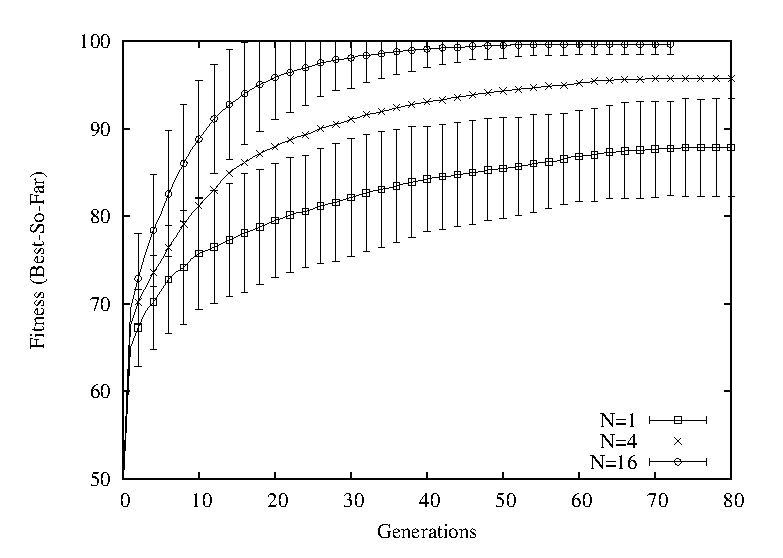
\includegraphics[width=3.25in]{maxones_cmla_collaborators_alpha_1_gens}&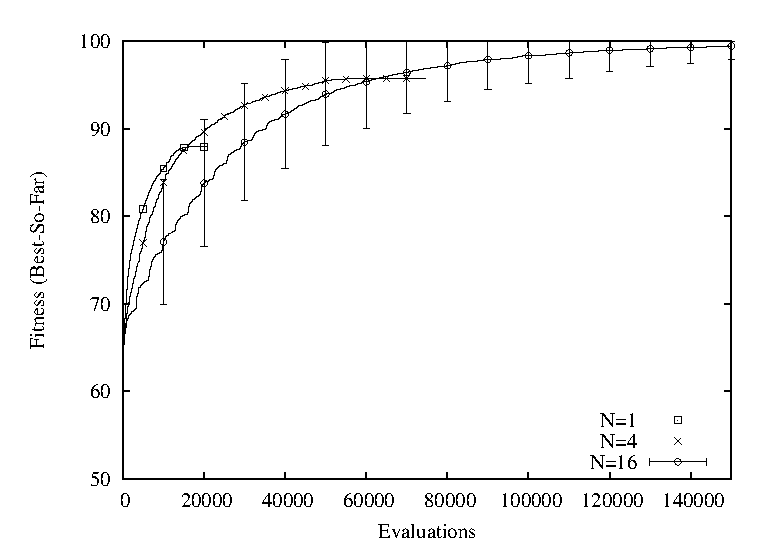
\includegraphics[width=3.25in]{maxones_cmla_collaborators_alpha_1_evals}\\
%	\end{tabular}
%	\label{fig:maxones_cmla_collaborators_alpha_1}

%	\caption{Best-so-far fitness versus number of (subfigure a) generations and (subfigure b) evaluations, for \(N\) collaborators, on a 100-bit \textsc{MaxOnes} problem where \(N=1\), \(N=4\), and \(N=16\). 95\% confidence interval bars on subfigure (b) omitted for clarity.}
%\end{figure}

\begin{figure}[t]
	\begin{center}
	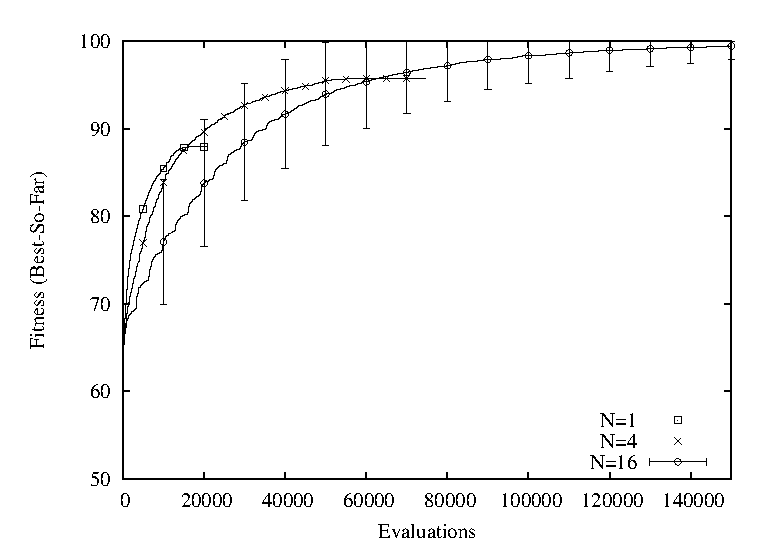
\includegraphics[width=3.3in]{maxones_cmla_collaborators_alpha_1_evals}
	\end{center}
	\caption{Mean best-so-far fitness versus number of evaluations, for \(\bm{N}\) collaborators, \(\bm{\alpha=1}\), on a 100-bit \textsc{MaxOnes} problem where \(\bm{N=1}\), \(\bm{N=4}\), and \(\bm{N=16}\).  Confidence intervals are omitted for clarity.}
	\vspace{-1em}
	\label{fig:maxones_cmla_collaborators_alpha_1}
\end{figure}

\subsection{Comparison and Results}

This section presents some of the simulation results for CEDA.  All experiments were averaged over 50 runs and use a tournament size of \(H=2\).\ignore{Because the number of evaluations would otherwise be unreasonably high, we set \(W=1\) in these experiments.}

From the theorem in Section \ref{proofs}, we expect the probability of convergence to the global optimum for the EGT model to increase with number of collaborators. We likewise expect to see a similar effect as we increase the number of collaborators in CEDA. Figure \ref{fig:maxones_cmla_collaborators_alpha_1} plots the convergence trajectory of CEDA with 1, 4, and 16 collaborators on {\sc MaxOnes},  using the definition:

%\vspace{-1em}
\begin{defn}{\textsc{MaxOnes}: $\{0,1\}^n \rightarrow \mathbb{R}$ is defined as:} \(\textsc{MaxOnes}(x) = \sum_i^n x_i\) .\end{defn}
%\vspace{-1em}

We observe that the solution quality improves as \(N\) increases: without a sufficiently large value of \(N\), CEDA converges too rapidly, and ultimately prematurely, even on as simple a problem as {\sc MaxOnes}.  The differences in means shown are highly statistically significant: using an unknown-variance 2-tailed {\it t}-test, all \(p-\) values are less than \(10^{-15}\).

\begin{figure}[t]
\begin{center}
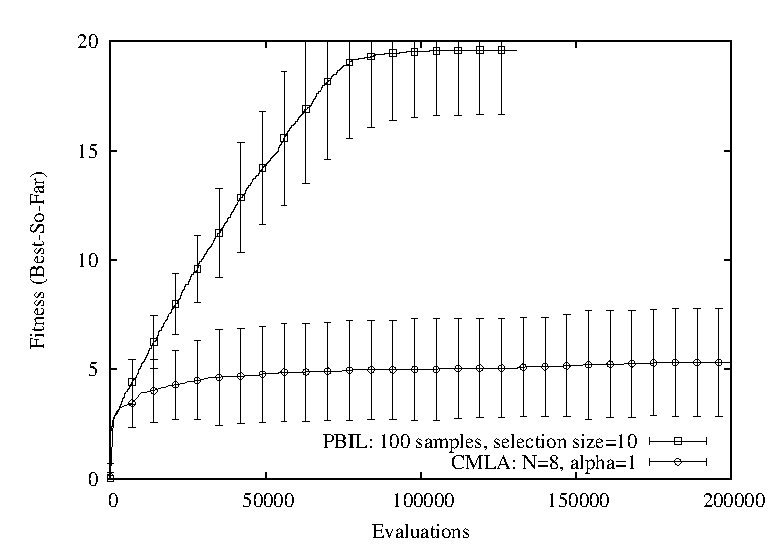
\includegraphics[width=3.3in]{lobproblem_pbil_vs_cmla_8_alpha_1_evals}
\end{center}
\caption{Best-so-far trajectory versus number of evaluations for
\textsc{LeadingOnesBlocks} problem, 100 bits, 5-bit blocks (so that the ideal fitness is 20). PBIL (100 samples, selection size 10, \(\bm{\alpha=0.005}\)) is compared to CEDA (\(\bm{H=2, N=8, \alpha=1}\)). Bars show 95\% confidence intervals.}
\label{fig:lobproblem_pbil_vs_cmla_8_alpha_1_evals}
\vspace{-0.5em}
\end{figure}

\ignore{However, a moderately large value of \(N\) may not be enough, particularly with the small sample due to \(W=1\).  }We then compared CEDA with one univariate EDA (namely, PBIL) on the {\sc LeadingOnesBlocks} problem, defined as:

%\vspace{-1em}
\begin{defn}{For $n \in \mathbb{R}$ and $b \in \{1,...,n\}$ so that $n/b \in \mathbb{N}$, $\textsc{LeadingOnesBlocks}_b: \{0,1\}^n \rightarrow \mathbb{R}$ is defined as:} \(\textsc{LeadingOnesBlocks}_b(x) = \sum_{i=1}^{n/b} \prod_{j=1}^{b \cdot i} x_j \)\quad .\end{defn}
%\vspace{-1em}

Figure \ref{fig:lobproblem_pbil_vs_cmla_8_alpha_1_evals} shows the results for the two, with \(H=2, N=8, \alpha=1\) for CEDA, and PBIL set to 100 samples, with a selection size of 10.  CEDA clearly does not converge to the optimum fitness.  (Very highly statistically significant with \(p<10^{-65}\)).  Rather than dramatically increase the number of samples (\(N\)) in CEDA to achieve an optimal solution quality, we chose instead to apply a probability update rule (\(\alpha < 1\)) that is similar to the one used in PBIL, thus only gradually mixing in new values to the population distributions.  Experiment suggests that a good value for CEDA is \(\alpha=0.05\).  Figure \ref{fig:lobproblem_pbil_vs_cmla_8_alpha_0p05_evals} shows the results after applying \(\alpha=0.05\) to CEDA with \(N=8\). Using a smaller learning rate in this manner helps CEDA to achieve the optimal solution.

\begin{figure}[t]
\begin{center}
\includegraphics[width=3.3in]{lobproblem_pbil_vs_cmla_8_alpha_0p05_evals}
\end{center}
\caption{Best-so-far trajectory versus number of evaluations for
\textsc{LeadingOnesBlocks} problem, 100 bits, 5-bit blocks (so that the ideal fitness is 20). PBIL (100 samples, selection size 10, \(\bm{\alpha=0.005}\)) is compared to CEDA (\(\bm{H=2, N=8, \alpha=0.05}\)).  Bars show 95\% confidence intervals (omitted on PBIL for clarity, see Figure \ref{fig:lobproblem_pbil_vs_cmla_8_alpha_1_evals} instead.}
\label{fig:lobproblem_pbil_vs_cmla_8_alpha_0p05_evals}
\end{figure}

However, as the figures indicate, CEDA is still wasteful in terms of the number of evaluations.  In Section \ref{edacceamodel} we noted that CEDA can be very inefficient as we construct and evaluate at least \(N\) unique individuals for {\it every single allele}, but do not reuse our results to inform the distributions for the other alleles.  Figure \ref{fig:lobproblem_pbil_vs_cmla_8_alpha_0p05_evals} illustrates this problem.

The wastefulness of CEDA in terms of evaluations is bad news in practice, since we have found that CEDA quickly gets trapped in local optima on some problems when the number of collaborators is insufficient.  We've found similar results on related test problems.

\section{Conclusion}

As it turns out, univariate EDAs and CCEAs are very similar methods.  The standard univariate EDA data model is essentially identical to the CCEA infinite-population EGT model.  Given this, it is possible to transfer theory and algorithms from CCEAs to EDAs and vice versa.  As an example, we have extended an existing CCEA theoretical result, originally for the 2-population CCEA case, to the \(M\)-population case.  This result shows that a given CCEA algorithm can be made to converge with a probability of \(1-\epsilon\) for any desired setting of \(\epsilon\) regardless of the problem.  We then transferred this result to the univariate EDA framework as well, demonstrating an EDA algorithm that approximates the theoretical model.  However, the algorithm is very expensive in terms of evaluations, and as expected, it does not perform well compared to PBIL, one of several common univariate EDA algorithms.

We believe this example serves as an illustration of what might be possible given the connection between these two techniques.  This opens up many avenues for future work.  For example, how would CCEA-style marginal ``population'' sample distributions compare to EDA-style marginal distributions?  Could we convert algorithms such as CGA, PBIL, or UMDA to operate in the sample-distribution situation of CCEAs?  Can further theory from either side inform the other?  What would the equivalent of BOA be in a CCEA context?  And importantly: are there other disparate methods which might actually be closely related?

\section{Proofs}
\label{proofs}

As discussed in Section \ref{egt}, it has been shown that a two-population cooperative coevolutionary EGT model, with tournament selection, and with maximum-of-\(M\)-collaborations fitness assessment, will converge to the optimum within some \(\epsilon\) probability given a sufficiently large value of \(M\).  This model is the one described by Equations  \ref{tournamentselection} and \ref{maxofn}.  The theorem here extends this convergence proof to an \(N\)-population cooperative coevolutionary Evolutionary Game Theory model.


\paragraph{Notation} For the following proof, we apply the same notation used in Section \ref{edacceamodel}. We describe it again here, for clarity.

We use $X_p$ to denote the space of genotypes of the $p$-th population.  For simplicity, we have $X_p = \left\{1, 2, 3, ..., n_p \right\}$ where $n_p$ is the number of genotypes for the $p$-th population.  For each population $p$ from $1$ to $M$, and for each genotype $i$ from $1$ to $n_p$, we let ${_p}x^{(t)}_i$ denote the ratio of individuals with genotype $i$ in population $p$ at generation $t$.  We further define $Y_{p} = X_1 \times  ... \times X_{p-1} \times X_{p+1} \times ... \times X_M$ as the joint space of all possible collaborators for an individual from population $p$ (notice that \(X_p\) is missing).  

\onecolumn 

\begin{multicols}{2}

Here we will deviate from our previous equations in our use of \(j\).  Now \(j\) will represent a {\it tuple} of genotypes chosen from various populations to collaborate with genotype \(i\).

We will also extend \({_p}y_j\) to refer not to the proportion of genotype \(j\) in the second population (as was the case earlier) but rather to the proportion of collaborating tuple \(j\) in the joint collaboration space.  That is, for tuple $j \in Y_{p}$ with $j = \left( j_1, ..., j_{p-1}, j_{p+1}, ..., j_M \right)$, we use the notation ${_p}y^{(t)}_j = \prodc{v=1..M: v \ne p} {_v}x^{(t)}_{j_v}$.  Likewise, $a_{i j}$ is the reward for genotype $i$ when combined with collaborators in tuple $j$.

Likewise for clarity, we repeat Equations \ref{approx_eqn1} and \ref{approx_eqn2}, which describe the formal model for CCEAs with \(N\) individuals.  For each population \(p\) and each genotype \(i \in p\):
\end{multicols}

\vspace{-1em}
\begin{equation}
{_p}u^{(t)}_i =\suma{j \in Y_{p}} a_{i j} \frac{{_p}y^{(t)}_j}{\sumb{k \in Y_{p}}{a_{i k} = a_{i j}} {_p}y^{(t)}_k}  \left(  \left (\sumb{k \in Y_{p}}{a_{i k} \leq a_{i j} } {_p}y^{(t)}_k \right)^N - \left( \sumb{k \in Y_{p}}{a_{i k} < a_{i j} } {_p}y^{(t)}_k  \right)^N \right ) 
\end{equation}

\begin{equation}
{_p}x^{(t+1)}_i  = \frac{{_p}x^{(t)}_i}{\sumb{k \in X_{p}}{{_p}u^{(t)}_k = {_p}u^{(t)}_i} {_p}x^{(t)}_k} \left ( \left(  \sumb{k \in X_{p}}{{_p}u^{(t)}_k \leq {_p}u^{(t)}_i} {_p}x^{(t)}_k  \right)^H - \left( \sumb{k \in X_{p}}{{_p}u^{(t)}_k < {_p}u^{(t)}_i} {_p}x^{(t)}_k \right)^H \right )
\end{equation}

\ignore{
\vspace{0.3in}
\noindent\begin{eqnarray}
{_p}u^{(t)}_i & = & \suma{j \in Y_{p}} { a_{i j} \frac{{_p}y^{(t)}_j}{\sumb{k \in Y_{p}}{a_{i k} = a_{i j}} {_p}y^{(t)}_k} \left( \left( \sumb{k \in Y_{p}}{a_{i k} \leq a_{i j} } {_p}y^{(t)}_k \right)^N - \left( \sumb{k \in Y_{p}}{a_{i k} < a_{i j} } {_p}y^{(t)}_k \right)^N \right) } \label{approx_eqn1}\\
{_p}x^{(t+1)}_i  & = & \frac{{_p}x^{(t)}_i}{\sumb{k \in X_{p}}{{_p}u^{(t)}_k = {_p}u^{(t)}_i} {_p}x^{(t)}_k} \left( \left( \sumb{k \in X_{p}}{{_p}u^{(t)}_k \leq {_p}u^{(t)}_i} {_p}x^{(t)}_k \right)^H - \left( \sumb{k \in X_{p}}{{_p}u^{(t)}_k < {_p}u^{(t)}_i} {_p}x^{(t)}_k \right)^H \right) \label{approx_eqn2}
\end{eqnarray}
}

\begin{multicols}{2}

%\vspace{0.2in}
%\begin{multicols}{2}
%\noindent for each population $p$ and each genotype $i$ in $p$.
\begin{lemma}
Assume the populations for the EGT model are initialized at random based on a uniform distribution over all possible initial populations.  Then, for any $\epsilon>0$, there exists $\theta_\epsilon>0$ such that

\begin{eqnarray}
& P\left( \min_{i=1..n_p} {_p}x^{(0)}_i \leq \theta_\epsilon \right) < \epsilon \label{ineq1}\\
& P\left( \max_{i=1..n_p} {_p}x^{(0)}_i \geq 1-\theta_\epsilon \right) < \epsilon \label{ineq2}
\end{eqnarray}

for all populations $p$ from $1$ to $M$.\end{lemma}

\begin{proof}
One method to sample the simplex $\Delta^n$ uniformly is described in \cite{devroye86nonuniform} (pages 568--569): take $n-1$ uniformly distributed numbers in $\left[0,1\right]$, sort them, and use the differences between consecutive numbers (also, the difference between the smallest number and $0$, and the difference between $1$ and the largest number) as the coordinates for the point.  

Let $p$ be an arbitrary population from $1$ to $M$.  It follows that %$\left({_p}x^{(0)}_i\right)_{i=1..n_p}$ 
$({_p}x^{(0)}_i)_{i=1..n_p}$
can be generated as the difference between $n-1$ numbers generated uniformly in the range $\left[0,1\right]$.  It then follows that $\min_{i=1..n} {_p}x^{(0)}_i$ is the closest distance between two such numbers (and possibly including the boundaries $0$ and $1$).

Suppose $\gamma>0$ is a sufficiently small number.  We iterate over the $n_p - 1$ uniformly-distributed random numbers that are needed to generate an initial population $({_p}x^{(0)}_i)_{i=1..n_p}$.  The probability that the first number is not within $\gamma$ of the boundaries $0$ and $1$ is $1-2\gamma$.  The probability that the second number is not within $\gamma$ of the boundaries, or of the first number, is less than or equal to $1-4\gamma$.  In general, the probability that the $k$th number is not within $\gamma$ of the boundaries, or of the first $k-1$ numbers, is less than or equal to $1-2 k \gamma$.  Since the numbers are generated independently of one another, the probability that the closest pair of points (considering the boundaries) is farther apart than $\gamma$ is:
\vspace{1em}
\begin{eqnarray*}
\begin{aligned}
P\left( \min_{i=1..n_p} {_p}x^{(0)}_i \leq \gamma \right)
&= 1 - P\left( \min_{i=1..n_p} {_p}x^{(0)}_i > \gamma \right)\\
&= 1 - \prod^{n_p - 1}_{i=1} \left( 1-2 i \gamma \right) \quad\\
&\leq \quad 1 - \left( 1 - 2 \left(n_p - 1\right) \gamma \right)^{n_p - 1}\\
&\leq \quad 1 - \left( 1 - 2 \left(n_{p^*} - 1\right) \gamma \right)^{n_{p^*} - 1}
\end{aligned}
\end{eqnarray*}

\noindent where $n_{p^*} = \max_{i=1..M} n_i$.  Given that

\begin{eqnarray*}
\lim_{\gamma \rightarrow 0} 1 - \left( 1 - 2 \left(n_{p^*} - 1\right) \gamma \right)^{n_{p^*} - 1} & = & 0
\end{eqnarray*}

\noindent it follows that for any $\epsilon>0$ there exists $\theta_\epsilon>0$ such that $P( \min_{i=1..n_p} {_p}x^{(0)}_i \leq \theta_\epsilon) < \epsilon$ for all populations $p_1 ... p_M$. %from $1$ to $M$.

To prove Inequality~\ref{ineq2}, note that \mbox{$\max_{i=1..n_p} {_p}x^{(0)}_i \geq 1-\theta_\epsilon$} implies that all other ${_p}x_i$ ratios except for the maximum are smaller than $\theta_\epsilon$, which, as proven above, occurs with probability smaller than $\epsilon$.
\end{proof}

\begin{lemma}
Assume the populations for the EGT model are initialized at random based on a uniform distribution over all possible initial populations.  Then, for any $\epsilon>0$, there exists $\eta_\epsilon>0$ such that

\[
\begin{split}
&P\left( \min_{p=1..M} \min_{i=1..n_p} {_p}x^{(0)}_i > \eta_\epsilon \wedge \max_{p=1..M} \max_{i=1..n_p} {_p}x^{(0)}_i < 1-\eta_\epsilon\right)\\
&\qquad\qquad\geq 1 - \epsilon
\end{split}
\]
\renewcommand{\qed}{ }

In other words, there is an arbitrary probability that the initial populations contain reasonable values (not too close to either $0$ or $1$) for all proportions of genotypes.
\end{lemma}


\begin{proof}
We apply Lemma 1 for $\frac{1-\sqrt[M]{1-\epsilon}}{2}$, which is greater than 0.  The specific value of $\eta_\epsilon$ for this proof equals the value of $\theta_\frac{1-\sqrt[M]{1-\epsilon}}{2}$ from Lemma 1.  It follows that:
\renewcommand{\qed}{ }
\end{proof}

\end{multicols}

\begin{eqnarray*}
& P\left( \min_{p=1..M} \min_{i=1..n_p} {_p}x^{(0)}_i > \eta_\epsilon \wedge \max_{p=1..M} \max_{i=1..n_p} {_p}x^{(0)}_i < 1-\eta_\epsilon \right)\\
& = \prodc{p=1..M} P \left( \min_{i=1..n_p} {_p}x^{(0)}_i > \theta_\frac{1-\sqrt[M]{1-\epsilon}}{2} \wedge \max_{i=1..n_p} {_p}x^{(0)}_i < 1-\theta_\frac{1-\sqrt[M]{1-\epsilon}}{2} \right) \\
&  =  \prodc{p=1..M} \left( 1 - P \left( \min_{i=1..n_p} {_p}x^{(0)}_i \leq \theta_\frac{1-\sqrt[M]{1-\epsilon}}{2} \vee \max_{i=1..n_p} {_p}x^{(0)}_i \geq 1-\theta_\frac{1-\sqrt[M]{1-\epsilon}}{2} \right) \right)\\
& \geq \prodc{p=1..M} \left( 1 - \left( P \left( \min_{i=1..n_p} {_p}x^{(0)}_i \leq \theta_\frac{1-\sqrt[M]{1-\epsilon}}{2} \right) + P \left( \max_{i=1..n_p} {_p}x^{(0)}_i \geq 1-\theta_\frac{1-\sqrt[M]{1-\epsilon}}{2} \right) \right) \right)\\
& \geq \prodc{p=1..M} \left( 1 - 2 \frac{1-\sqrt[M]{1-\epsilon}}{2} \right) \\
& = 1 - \epsilon \qquad \qquad \qed
\end{eqnarray*}

\begin{multicols}{2}
\begin{theorem}
Given a joint reward system with a unique global optimum $a_{i_1^\star i_2^\star ... i_M^\star}$, for any $\epsilon > 0$ and any $H \geq 2$, there exists a value $N_\epsilon \geq 1$ such that the theoretical CCEA model in Equations~\ref{approx_eqn1}--\ref{approx_eqn2} converges to the global optimum with probability greater than $\left(1-\epsilon\right)$ for any number of collaborators $N$ such that $N \geq N_\epsilon$.\end{theorem}

\begin{proof}
We only use $\epsilon$ as a guarantee for the worst case scenario for the proportions of individuals in the initial populations.  From Lemma~2, it follows that there exists $\eta_\epsilon>0$ such that with probability at least $1-\epsilon$, it holds that $\eta_\epsilon < {_p}x^{(0)}_i < 1 - \eta_\epsilon$ for all genotypes $i$ in all populations $p$.  In other words, with probability $\epsilon$, the initial populations will not have any proportion of individuals that cover more than $1-\eta_\epsilon$, nor cover less than $\eta_\epsilon$ of the entire population.

We will prove that there exists \mbox{$N_\epsilon \geq 0$} such that the EGT model converges to the global optimum for any $N \geq N_\epsilon$ and for all initial configurations that satisfy \mbox{$\eta_\epsilon < {_p}x^{(0)}_{i^\star} < 1 - \eta_\epsilon$} for all populations $p$.  To this end, let $\alpha$ be the second highest element joint reward ($\alpha < a_{i^* j^*}$).    It follows that ${_p}u^{(t)}_i \leq \alpha$ for all $i \neq i^\star$ in all populations $p$. This is because (by refining Equation~\ref{approx_eqn1}):
\renewcommand\qed{}
\end{proof}
\end{multicols}

\vspace{-4em}
\noindent\begin{eqnarray*}
{_p}u^{(t)}_i & = & \suma{j \in Y_{p}} { a_{i j} \frac{{_p}y^{(t)}_j}{\sumb{k \in Y_{p}}{a_{i k} = a_{i j}} {_p}y^{(t)}_k} \left( \left( \sumb{k \in Y_{p}}{a_{i k} \leq a_{i j} } {_p}y^{(t)}_k \right)^N - \left( \sumb{k \in Y_{p}}{a_{i k} < a_{i j} } {_p}y^{(t)}_k \right)^N \right) }\\
{_p}u^{(t)}_i & \leq & \suma{j \in Y_{p}} { \alpha \frac{{_p}y^{(t)}_j}{\sumb{k \in Y_{p}}{a_{i k} = a_{i j}} {_p}y^{(t)}_k} \left( \left( \sumb{k \in Y_{p}}{a_{i k} \leq a_{i j} } {_p}y^{(t)}_k \right)^N - \left( \sumb{k \in Y_{p}}{a_{i k} < a_{i j} } {_p}y^{(t)}_k \right)^N \right) }\\
& \leq & \alpha \suma{j \in Y_{p}} { \left( \left( \sumb{k \in Y_{p}}{a_{i k} \leq a_{i j} } {_p}y^{(t)}_k \right)^N - \left( \sumb{k \in Y_{p}}{a_{i k} < a_{i j} } {_p}y^{(t)}_k \right)^N \right) } \leq \alpha
\end{eqnarray*}

Next, we work on identifying a lower bound for ${_p}u^{(t)}_{i_p^\star}$.  For simplicity, let $i^*$ stand for $i_p^*$, and $j^*$ stand for the optimal tuple of collaborators for $i^*$.

\noindent\begin{eqnarray*}
{_p}u^{(t)}_{i^\star} & = & \suma{j \in Y_{p}} { a_{i^\star j} \frac{{_p}y^{(t)}_j}{ \sumb{k \in Y_{p}}{a_{i^\star k} = a_{i^\star j}} {_p}y^{(t)}_k } \left( \left( \sumb{k \in Y_{p}}{a_{i^\star k} \leq a_{i^\star j} } {_p}y^{(t)}_k \right)^N - \left( \sumb{k \in Y_{p}}{a_{i^\star k} < a_{i^\star j} } {_p}y^{(t)}_k \right)^N \right) }\\
& = & a_{i^* j^*} \left( 1 - \left( 1 - {_p}y^{(t)}_{j^\star} \right) ^N \right) +\\
& & \sumb{j \in Y_{p}}{j \neq j^\star} { a_{i^\star j} \frac{{_p}y^{(t)}_j}{ \sumb{k \in Y_{p}}{a_{i^\star k} = a_{i^\star j} } {_p}y^{(t)}_k} \left( \left( \sumb{k \in Y_{p}}{a_{i^\star k} \leq a_{i^\star j} } {_p}y^{(t)}_k \right)^N - \left( \sumb{k \in Y_{p}}{a_{i^\star k} < a_{i^\star j} } {_p}y^{(t)}_k \right)^N \right) }
\end{eqnarray*}

\vspace{10in}
\noindent We further refine the lower bound for ${_p}u^{(t)}_{i^\star}$:


\noindent\begin{eqnarray*}
{_p}u^{(t)}_{i^\star} & = & a_{i^* j^*} \left( 1 - \left( 1 - {_p}y^{(t)}_{j^\star} \right) ^N \right) +\\
& & \sumb{j \in Y_{p}}{j \neq j^\star \wedge a_{i^\star j} \geq 0} { a_{i^\star j} \frac{{_p}y^{(t)}_j}{ \sumb{k \in Y_{p}}{a_{i^\star k} = a_{i^\star j} } {_p}y^{(t)}_k} \left( \left( \sumb{k \in Y_{p}}{a_{i^\star k} \leq a_{i^\star j} } {_p}y^{(t)}_k \right)^N - \left( \sumb{k \in Y_{p}}{a_{i^\star k} < a_{i^\star j} } {_p}y^{(t)}_k \right)^N \right) }+\\
& & \sumb{j \in Y_{p}}{j \neq j^\star \wedge a_{i^\star j} < 0} { a_{i^\star j} \frac{{_p}y^{(t)}_j}{ \sumb{k \in Y_{p}}{a_{i^\star k} = a_{i^\star j} } {_p}y^{(t)}_k} \left( \left( \sumb{k \in Y_{p}}{a_{i^\star k} \leq a_{i^\star j} } {_p}y^{(t)}_k \right)^N - \left( \sumb{k \in Y_{p}}{a_{i^\star k} < a_{i^\star j} } {_p}y^{(t)}_k \right)^N \right) }\\
& \geq & a_{i^* j^*} \left( 1 - \left( 1 - {_p}y^{(t)}_{j^\star} \right) ^N \right) +\\
& & \sumb{j \in Y_{p}}{j \neq j^\star \wedge a_{i^\star j} < 0} { a_{i^\star j} \frac{ {_p}y^{(t)}_j}{ \sumb{k \in Y_{p}}{a_{i^\star k} = a_{i^\star j} } {_p}y^{(t)}_k} \left( \left( \sumb{k \in Y_{p}}{a_{i^\star k} \leq a_{i^\star j} } {_p}y^{(t)}_k \right)^N - \left( \sumb{k \in Y_{p}}{a_{i^\star k} < a_{i^\star j} } {_p}y^{(t)}_k \right)^N \right) }\\
& \geq & a_{i^* j^*} \left( 1 - \left( 1 - {_p}y^{(t)}_{j^\star} \right) ^N \right) + \sumb{j \in Y_{p}}{j \neq j^\star \wedge a_{i^\star j} < 0} { a_{i^\star j} \frac{ {_p}y^{(t)}_j}{ \sumb{k \in Y_{p}}{a_{i^\star k} = a_{i^\star j} } {_p}y^{(t)}_k} \left( \sumb{k \in Y_{p}}{a_{i^\star k} \leq a_{i^\star j} } {_p}y^{(t)}_k \right)^N }
\end{eqnarray*}


Given that $\sumd{k=1}{m} {_p}y^{(t)}_k = 1$, we further refine the previous inequality:


\noindent\begin{eqnarray}
\nonumber {_p}u^{(t)}_{i^\star} & \geq & a_{i^* j^*} \left( 1 - \left( 1 - {_p}y^{(t)}_{j^\star} \right) ^N \right) + \sumb{j \in Y_{p}}{j \neq j^\star \wedge a_{i^\star j} < 0} { a_{i^\star j} \frac{ {_p}y^{(t)}_j}{ \sumb{k \in Y_{p}}{a_{i^\star k} = a_{i^\star j} } {_p}y^{(t)}_k} \left( 1 - {_p}y^{(t)}_{j^\star} \right)^N }\\
\nonumber & \geq & a_{i^* j^*} \left( 1 - \left( 1 - {_p}y^{(t)}_{j^\star} \right) ^N \right) + \left( 1 - {_p}y^{(t)}_{j^\star} \right)^N \sumb{j \in Y_{p}}{j \neq j^\star \wedge a_{i^\star j} < 0} { a_{i^\star j} }\\
& = & a_{i^* j^*} - \left( 1 - {_p}y^{(t)}_{j^\star} \right) ^N \left( a_{i^* j^*}  - \sumb{j \in Y_{p}}{j \neq j^\star \wedge a_{i^\star j} < 0} { a_{i^\star j} } \right)\\
& = & a_{i^* j^*} - \left( 1 - \prodb{r=1..M}{r \ne p} {_r}x^{(t)}_{j_r^\star} \right) ^N \left( a_{i^* j^*}  - \sumb{j \in Y_{p}}{j \neq j^\star \wedge a_{i^\star j} < 0} { a_{i^\star j} } \right) \label{u_i:star:bounds}
\end{eqnarray}


The inequalities $\eta_\epsilon < {_r}x^{(0)}_{j_r^\star} < 1 - \eta_\epsilon$ hold for all initial populations $r$, as inferred earlier from Lemma~2.  It follows from Equation~\ref{u_i:star:bounds} that:


\noindent\begin{eqnarray}
{_p}u^{(0)}_{i^\star} & \geq & a_{i^\star j^\star} - \left( 1 - {\eta_\epsilon}^{M-1} \right) ^N \left( a_{i^\star j^\star}  - \laxsumb{j \in Y_{p}}{j \neq j^\star \wedge a_{i^\star j} < 0} { a_{i^\star j} } \right) \label{u_i:star:lower:bound}
\end{eqnarray}

\vspace{10in}
\begin{multicols}{2}
\noindent However,

\begin{equation}
\lim_{N \rightarrow \infty} a_{i^\star j^\star} - \left( 1 - {\eta_\epsilon}^{M-1} \right) ^N \left( a_{i^\star j^\star}  - \laxsumb{j \in Y_{p}}{j \neq j^\star \wedge a_{i^\star j} < 0} { a_{i^\star j} } \right) \quad = \quad a_{i^\star j^\star} \label{u_i:star:lim2}
\end{equation}

\vspace{0.5em}Given that $a_{i^\star j^\star} > \alpha$, Equation~\ref{u_i:star:lim2} implies that there exists $N_p \geq 1$ such that

\begin{equation}
a_{i^\star j^\star} - \left( 1 - {\eta_\epsilon}^{M-1} \right) ^N \left( a_{i^\star j^\star}  - \laxsumb{j \in Y_{p}}{j \neq j^\star \wedge a_{i^\star j} < 0} { a_{i^\star j} } \right) > \alpha \label{lim:inf:greater:alpha}
\end{equation}

\vspace{0.5em}\noindent for all $N \geq N_p$.  From Equations~\ref{u_i:star:bounds} and \ref{lim:inf:greater:alpha}, it follows that ${_p}u^{(0)}_{i^\star} > \alpha$ for all $N \geq N_p$.  Observe that $N_p$ does not depend on the initial population $p$ we considered this far.

Let $N_\epsilon = \max_{p=1..M} \left( N_p \right)$, and let $N \geq N_\epsilon$.  Next, we show by induction by $t$ (the number of iterations of the model, i.e. the number of generations) that the following inequalities hold for all populations $p$:

\begin{eqnarray*}
{_p}u^{(t)}_{i^\star} & \geq & a_{i^\star j^\star} - \left( 1 - {\eta_\epsilon}^{M-1} \right) ^N \left( a_{i^\star j^\star}  - \laxsumb{j \in Y_{p}}{j \neq j^\star \wedge a_{i^\star j} < 0} { a_{i^\star j} } \right)\\
{_p}x^{(t+1)}_{i^\star} & \geq & {_p}x^{(t)}_{i^\star}\\
\end{eqnarray*}

At the first generation ($t=0$), the first inequality holds (from Equation~\ref{u_i:star:lower:bound}).  For a population $p$, we combine this with the definition of $N$.  It follows that ${_p}u^{(0)}_{i^\star} > {_p}u^{(0)}_i$ for all $i \neq i^\star$.  As a consequence, ${_p}x^{(1)}_{i^\star} = 1 - ( 1 - {_p}x^{(0)}_{i^\star} )^H > {_p}x^{(0)}_{i^\star}$ (from Equation~\ref{approx_eqn1}).

To prove the inductive step, it follows from Equation~\ref{u_i:star:bounds} and from the inductive hypothesis that 

\noindent\begin{eqnarray*}
{_p}u^{(t+1)}_{i^\star} \!\!\!\!& \geq & \!\!\!\!a_{i^\star j^\star} - \left( 1 - {_p}y^{(t+1)}_{j^\star} \right) ^N \left( a_{i^\star j^\star}  - \laxsumb{j \in Y_{p}}{j \neq j^\star \wedge a_{i^\star j} < 0} { a_{i^\star j} } \right)\\
& \geq & \!\!\!\!a_{i^\star j^\star} - \left( 1 - {_p}y^{(t)}_{j^\star} \right) ^N \left( a_{i^\star j^\star}  - \laxsumb{j \in Y_{p}}{j \neq j^\star \wedge a_{i^\star j} < 0} { a_{i^\star j} } \right)\\
& \cdots &\\
& \geq & \!\!\!\!a_{i^\star j^\star} - \left( 1 - {_p}y^{(0)}_{j^\star} \right) ^N \left( a_{i^\star j^\star}  - \laxsumb{j \in Y_{p}}{j \neq j^\star \wedge a_{i^\star j} < 0} { a_{i^\star j} } \right)\\
& \geq & \!\!\!\!a_{i^\star j^\star} - \left( 1 - {\eta_\epsilon}^M-1 \right) ^N \left( a_{i^\star j^\star}  - \laxsumb{j \in Y_{p}}{j \neq j^\star \wedge a_{i^\star j} < 0} { a_{i^\star j} } \right)
\end{eqnarray*}

Given the definitions of $N$ and $\alpha$, this also implies that ${_p}u^{(t+1)}_{i^\star} > \alpha > {_p}u^{(t+1)}_{i}$ for all $i \neq i^\star$.  As a consequence, \mbox{${_p}x^{(t+1)}_{i^\star} = 1 - ( 1 - {_p}x^{(t)}_{i^\star})^H \geq {_p}x^{(t)}_{i^\star}$} (from Equation~\ref{approx_eqn1}).

Having shown that ${_p}x^{(t)}_{i^\star}$ are monotonically increasing for all populations $p$, and given that they are all bounded between $0$ and $1$, it follows that they each converge to some value.  Given that ${_p}u^{(t)}_{i^\star} > {_p}u^{(t)}_i$ for all $i \neq i^\star$ at each iteration, it follows that ${_p}x^{(t+1)}_{i^\star} = 1 - ( 1 - {_p}x^{(t)}_{i^\star} )^H$ at each iteration as well.  If ${_p}\bar{x}$ is the limit of the ${_p}x^{(t)}_{i^\star}$ values when $t$ goes to $\infty$, then ${_p}\bar{x} = 1 - \left( 1 - {_p}\bar{x} \right)^H$, which implies that ${_p}\bar{x}$ is either $0$ or $1$.  We can rule out the $0$ limit because the values of ${_p}x^{(t)}_{i^\star}$ are monotonically increasing and ${_p}x^{(0)}_{i^\star}>\eta_\epsilon$.  Thus, ${_p}x^{(t)}_{i^\star}$ converges to $1$ for all populations $p$. \qed

\bibliographystyle{abbrv}
\vspace{1em}\bibliography{foga09-eda}
\end{multicols}

\end{document}
